\documentclass{ximera}

\usepackage{epsfig}

\graphicspath{
  {./}
  {figures/}
}


\usepackage{morewrites}

%\newcounter{ccounter}
%\setcounter{ccounter}{1}
%\newcommand{\Chapter}[1]{\setcounter{chapter}{\arabic{ccounter}}\chapter{#1}\addtocounter{ccounter}{1}}

%\newcommand{\section}[1]{\section{#1}\setcounter{thm}{0}\setcounter{equation}{0}}

%\renewcommand{\theequation}{\arabic{chapter}.\arabic{section}.\arabic{equation}}
%\renewcommand{\thefigure}{\arabic{chapter}.\arabic{figure}}
%\renewcommand{\thetable}{\arabic{chapter}.\arabic{table}}

%\newcommand{\Sec}[2]{\section{#1}\markright{\arabic{ccounter}.\arabic{section}.#2}\setcounter{equation}{0}\setcounter{thm}{0}\setcounter{figure}{0}}

\newcommand{\Sec}[2]{\section{#1}}

\setcounter{secnumdepth}{2}
%\setcounter{secnumdepth}{1} 

%\newcounter{THM}
%\renewcommand{\theTHM}{\arabic{chapter}.\arabic{section}}

\newcommand{\trademark}{{R\!\!\!\!\!\bigcirc}}
%\newtheorem{exercise}{}

\newcommand{\dfield}{{\sf dfield9}}
\newcommand{\pplane}{{\sf pplane9}}

\newcommand{\EXER}{\section*{Exercises}}%\vspace*{0.2in}\hrule\small\setcounter{exercise}{0}}
\newcommand{\CEXER}{}%\vspace{0.08in}\begin{center}Computer Exercises\end{center}}
\newcommand{\TEXER}{} %\vspace{0.08in}\begin{center}Hand Exercises\end{center}}
\newcommand{\AEXER}{} %\vspace{0.08in}\begin{center}Hand Exercises\end{center}}

% BADBAD: \newcommand{\Bbb}{\bf}

\newcommand{\R}{\mbox{$\Bbb{R}$}}
\newcommand{\C}{\mbox{$\Bbb{C}$}}
\newcommand{\Z}{\mbox{$\Bbb{Z}$}}
\newcommand{\N}{\mbox{$\Bbb{N}$}}
\newcommand{\D}{\mbox{{\bf D}}}
\usepackage{amssymb}
%\newcommand{\qed}{\hfill\mbox{\raggedright$\square$} \vspace{1ex}}
%\newcommand{\proof}{\noindent {\bf Proof:} \hspace{0.1in}}

\newcommand{\setmin}{\;\mbox{--}\;}
\newcommand{\Matlab}{{M\small{AT\-LAB}} }
\newcommand{\Matlabp}{{M\small{AT\-LAB}}}
\newcommand{\computer}{\Matlab Instructions}
\newcommand{\half}{\mbox{$\frac{1}{2}$}}
\newcommand{\compose}{\raisebox{.15ex}{\mbox{{\scriptsize$\circ$}}}}
\newcommand{\AND}{\quad\mbox{and}\quad}
\newcommand{\vect}[2]{\left(\begin{array}{c} #1_1 \\ \vdots \\
 #1_{#2}\end{array}\right)}
\newcommand{\mattwo}[4]{\left(\begin{array}{rr} #1 & #2\\ #3
&#4\end{array}\right)}
\newcommand{\mattwoc}[4]{\left(\begin{array}{cc} #1 & #2\\ #3
&#4\end{array}\right)}
\newcommand{\vectwo}[2]{\left(\begin{array}{r} #1 \\ #2\end{array}\right)}
\newcommand{\vectwoc}[2]{\left(\begin{array}{c} #1 \\ #2\end{array}\right)}



\newcommand{\inv}{^{-1}}
\newcommand{\CC}{{\cal C}}
\newcommand{\CCone}{\CC^1}
\newcommand{\Span}{{\rm span}}
\newcommand{\rank}{{\rm rank}}
\newcommand{\trace}{{\rm tr}}
\newcommand{\RE}{{\rm Re}}
\newcommand{\IM}{{\rm Im}}
\newcommand{\nulls}{{\rm null\;space}}

\newcommand{\dps}{\displaystyle}
\newcommand{\arraystart}{\renewcommand{\arraystretch}{1.8}}
\newcommand{\arrayfinish}{\renewcommand{\arraystretch}{1.2}}
\newcommand{\Start}[1]{\vspace{0.08in}\noindent {\bf Section~\ref{#1}}}
\newcommand{\exer}[1]{\noindent {\bf \ref{#1}}}
\newcommand{\ans}{}
\newcommand{\matthree}[9]{\left(\begin{array}{rrr} #1 & #2 & #3 \\ #4 & #5 & #6
\\ #7 & #8 & #9\end{array}\right)}
\newcommand{\cvectwo}[2]{\left(\begin{array}{c} #1 \\ #2\end{array}\right)}
\newcommand{\cmatthree}[9]{\left(\begin{array}{ccc} #1 & #2 & #3 \\ #4 & #5 &
#6 \\ #7 & #8 & #9\end{array}\right)}
\newcommand{\vecthree}[3]{\left(\begin{array}{r} #1 \\ #2 \\
#3\end{array}\right)}
\newcommand{\cvecthree}[3]{\left(\begin{array}{c} #1 \\ #2 \\
#3\end{array}\right)}
\newcommand{\cmattwo}[4]{\left(\begin{array}{cc} #1 & #2\\ #3
&#4\end{array}\right)}

\newcommand{\Matrix}[1]{\ensuremath{\left(\begin{array}{rrrrrrrrrrrrrrrrrr} #1 \end{array}\right)}}

\newcommand{\Matrixc}[1]{\ensuremath{\left(\begin{array}{cccccccccccc} #1 \end{array}\right)}}



\renewcommand{\labelenumi}{\theenumi)}
\newenvironment{enumeratea}%
{\begingroup
 \renewcommand{\theenumi}{\alph{enumi}}
 \renewcommand{\labelenumi}{(\theenumi)}
 \begin{enumerate}}
 {\end{enumerate}\endgroup}



\newcounter{help}
\renewcommand{\thehelp}{\thesection.\arabic{equation}}

%\newenvironment{equation*}%
%{\renewcommand\endequation{\eqno (\theequation)* $$}%
%   \begin{equation}}%
%   {\end{equation}\renewcommand\endequation{\eqno \@eqnnum
%$$\global\@ignoretrue}}

%\input{psfig.tex}

\author{Martin Golubitsky and Michael Dellnitz}

%\newenvironment{matlabEquation}%
%{\renewcommand\endequation{\eqno (\theequation*) $$}%
%   \begin{equation}}%
%   {\end{equation}\renewcommand\endequation{\eqno \@eqnnum
% $$\global\@ignoretrue}}

\newcommand{\soln}{\textbf{Solution:} }
\newcommand{\exercap}[1]{\centerline{Figure~\ref{#1}}}
\newcommand{\exercaptwo}[1]{\centerline{Figure~\ref{#1}a\hspace{2.1in}
Figure~\ref{#1}b}}
\newcommand{\exercapthree}[1]{\centerline{Figure~\ref{#1}a\hspace{1.2in}
Figure~\ref{#1}b\hspace{1.2in}Figure~\ref{#1}c}}
\newcommand{\para}{\hspace{0.4in}}

\renewenvironment{solution}{\suppress}{\endsuppress}

\ifxake
\newenvironment{matlabEquation}{\begin{equation}}{\end{equation}}
\else
\newenvironment{matlabEquation}%
{\let\oldtheequation\theequation\renewcommand{\theequation}{\oldtheequation*}\begin{equation}}%
  {\end{equation}\let\theequation\oldtheequation}
\fi

\makeatother


\title{Least Squares Approximations}

\begin{document}
\begin{abstract}
\end{abstract}
\maketitle

  \label{S:LSA}

Let $W\subset\R^n$ be a subspace and $b\in\R^n$ be a vector.  In this
section we solve a basic geometric problem and investigate some of its
consequences.  The problem is:
\begin{quote}
Find the vector $\tilde{w}\in W$ that is the nearest vector in $W$ to $b$.
\end{quote}

\begin{definition} \rm \label{D:least_squares}
The vector $\tilde{w}$ in the subspace $W$ of $\R^n$ that is the nearest to the 
vector $b$ in $\R^n$ is called the \em{least squares approximation} of 
$b$ in $W$.
\end{definition} 

\begin{figure}[htb]
        \centerline{%
        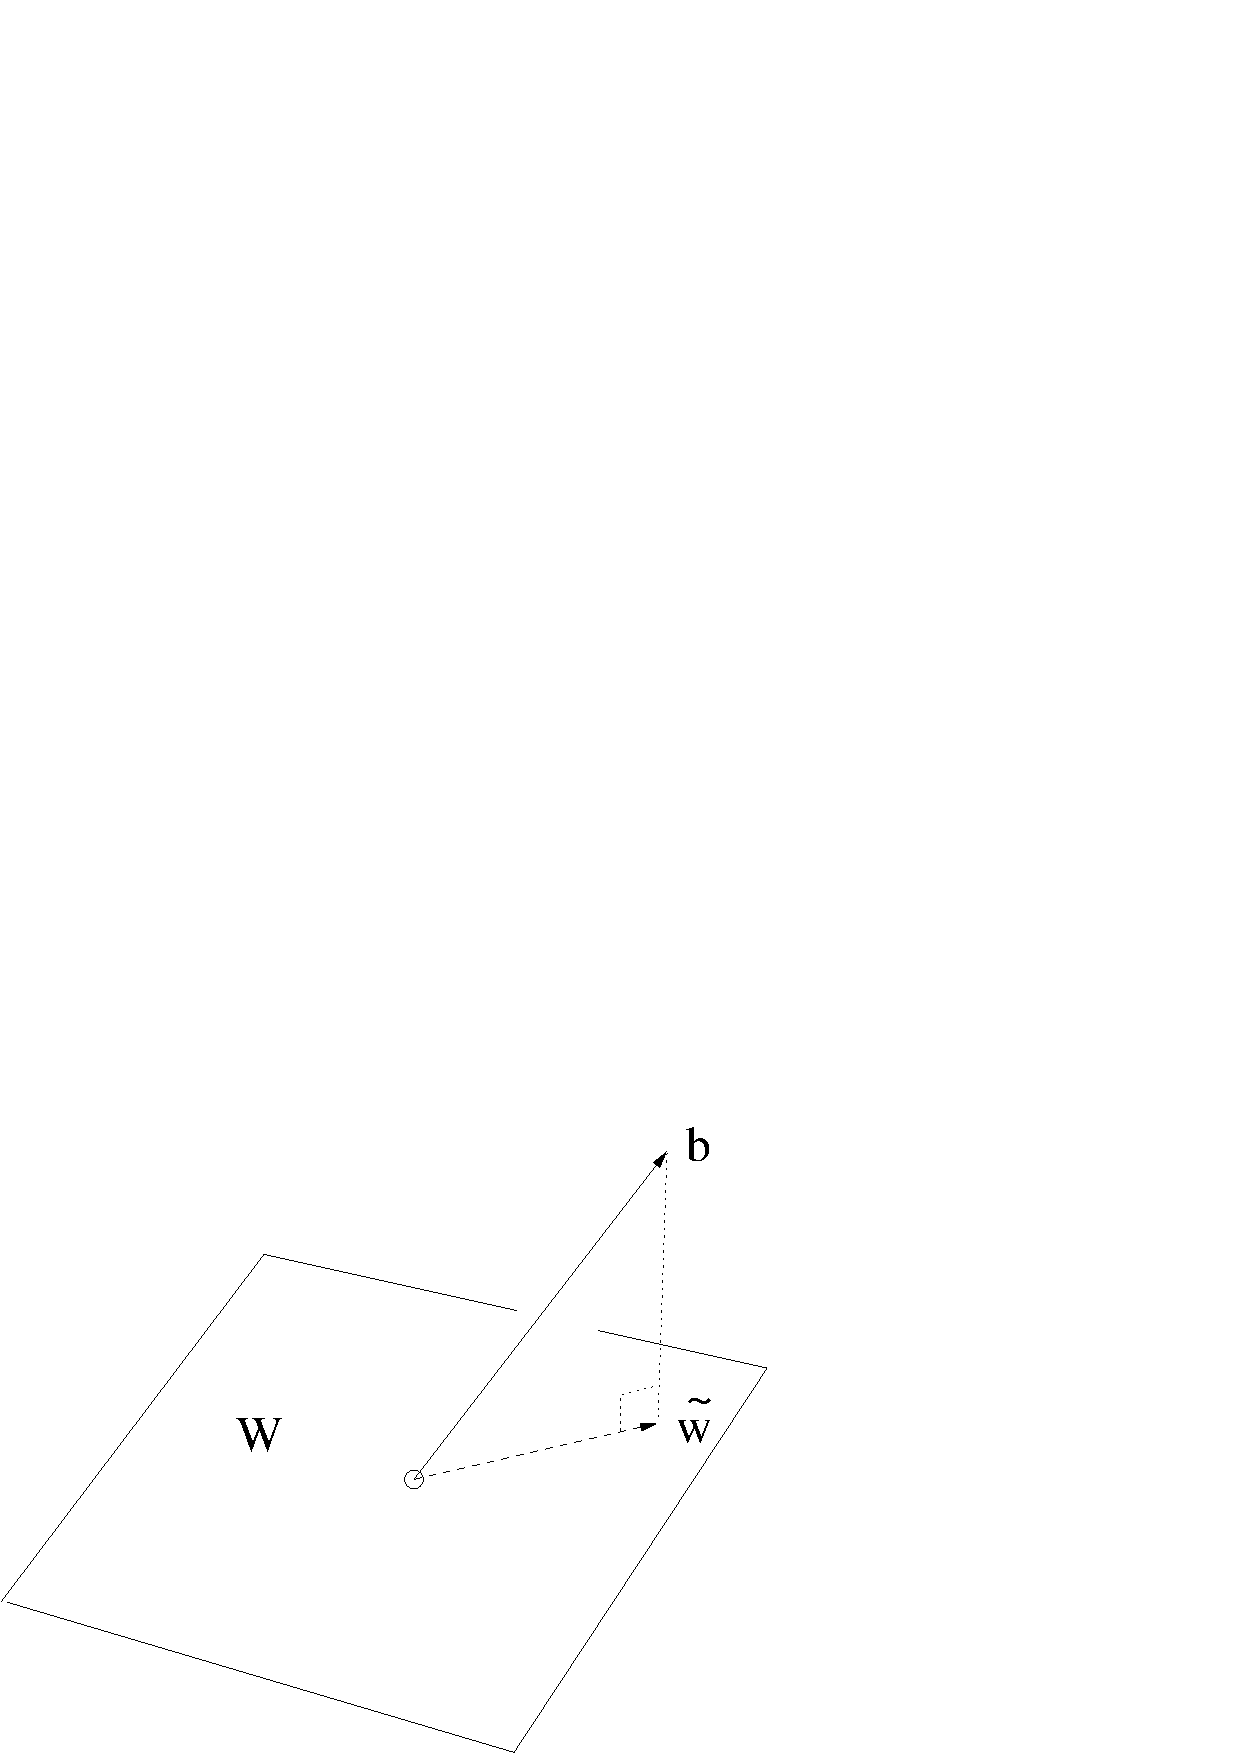
\includegraphics[width=2.5in]{../figures/nearest.pdf}}
        \caption{The vector $\tilde{w}$ is the least squares approximation of the vector $b$ by a vector in $W$.}
        \label{F:nearest}
\end{figure}


The distance between two vectors\index{distance!between vectors}
$v$ and $w$ is $||v-w||$.  Hence the least squares approximation 
can be rephrased as follows: find a vector $\tilde{w}\in W$ such that
\begin{equation}  \label{E:leastsq}
||b-\tilde{w}||\leq ||b-w|| \quad \forall w\in W.
\end{equation}
Condition \eqref{E:leastsq} is also called the
{\em least squares approximation}\index{least squares!approximation}.
In order to see where this name comes from \eqref{E:leastsq} can be 
rewritten in the equivalent form
\begin{equation} \label{E:LS_inequality}
||b-\tilde{w}||^2\leq ||b-w||^2 \quad \forall w\in W.
\end{equation}
The form \eqref{E:LS_inequality} means that the sum of the squares of the
components of the vectors $b - w$ is minimal at $w = \tilde{w}$.

Recall from \eqref{dotprod=0} that two vectors $z_1,z_2\in\R^n$ are perpendicular 
or equivalently {\em orthogonal} if $z_1\cdot z_2 = 0$.  Before continuing, we state and prove 
\begin{lemma}[The Law of Pythagorus] \index{Law of Pythagorus}  \label{L:LP}
The vectors $z_1,z_2\in\R^n$ are orthogonal if and only if  
\begin{equation} \label{E:LP}
||z_1+z_2||^2 = ||z_1||^2 + ||z_2||^2.
\end{equation}
\end{lemma}

\begin{proof}
To verify \eqref{E:LP} calculate 
\begin{align*}
  ||z_1+z_2||^2&=(z_1+z_2)\cdot(z_1+z_2) \\
  &=z_1\cdot z_1 +2z_1\cdot z_2+z_2\cdot z_2 \\
  &=||z_1||^2 + 2z_1\cdot z_2 +||z_2||^2.
\end{align*}
It follows that $z_1$ and $z_2$ satisfy \eqref{E:LP} if and only if $z_1\cdot z_2 = 0$  
if and only $z_1$ and $z_2$ are orthogonal.
\end{proof}

Using \eqref{E:leastsq} and \eqref{E:LP}, we can rephrase the minimum distance 
problem as follows.
\begin{lemma}  \label{L:orthoLSA}
The vector $\tilde{w}\in W$ is the closest vector to $b\in\R^n$ if the vector 
$b - \tilde{w}$ is orthogonal to every vector in $W$. See Figure~\ref{F:nearest}.
\end{lemma}

\begin{proof}  Write $b-w=z_1+z_2$ where $z_1=b-\tilde{w}$ and $z_2=\tilde{w}-w$.  By 
assumption, $b-\tilde{w}$ is orthogonal to every vector in $W$; so $z_1$ and 
$z_2\in W$ are orthogonal.  It follows from \eqref{E:LP} that
\[
||b-w||^2 = ||b-\tilde{w}||^2 + ||\tilde{w}-w||^2.
\]
Since $||\tilde{w}-w||^2\ge 0$, \eqref{E:leastsq} is valid, and $\tilde{w}$ is the 
vector in $W$ that is nearest to $b$. 
\end{proof}

\subsection*{Least Squares Distance to a Line}
\index{least squares!distance to a line}
\index{distance!to a line}

Suppose $W$ is as simple a subspace as possible; that is, suppose $W$ is one
dimensional with basis vector $w$.  Since $W$ is one dimensional, a vector
$\tilde{w}\in W$ that is closest to $b$ must be a multiple of $w$; that is,
$\tilde{w} = \alpha w$ for $\alpha\in\R$.  Suppose that we can find a scalar $a$ 
so that $b - \alpha w$ is orthogonal to every vector in $W$.  Then it follows from
Lemma~\ref{L:orthoLSA} that $\tilde{w}$ is the closest vector in $W$ to $b$.
To find $\alpha$, calculate
\[
0 = (b- \alpha w)\cdot w = b\cdot w - \alpha w\cdot w.
\]
Then
\[
\alpha = \frac{b\cdot w}{||w||^2}
\]
and
\begin{equation}  \label{E:singleortho}
\tilde{w} = \frac{b\cdot w}{||w||^2} w.
\end{equation}
Observe that $||w||^2\not=0$ since $w$ is a basis vector.

For example, if $b = (1,2,-1,3)\in\R^4$ and $w=(0,1,2,3)$.  The the vector
$\tilde{w}$ in the space spanned by $w$ that is nearest to $b$ is
\[
\tilde{w} = \frac{9}{14}w
\]
since $b \cdot w = 9$ and $||w||^2 = 14$.

\subsection*{Least Squares Distance to a Subspace}
\index{least squares!distance to a subspace}
\index{distance!to a subspace}

\ignore{
Similarly, using Lemma~\ref{L:orthoLSA} we can solve the general least
squares problem by solving a system of linear equations.  Let
$w_1,\ldots,w_k$ be a basis for $W$ and suppose that
\[
\tilde{w} = \alpha_1w_1 + \cdots + \alpha_kw_k
\]
for some scalars $\alpha_i$.  We now show how to find these scalars.
}
Similarly, we solve the general least squares problem by solving a 
system of linear equations.


\begin{theorem}  \label{T:nearestvector}
Let $b\in\R^n$ be a vector, let $\{w_1,\ldots,w_k\}$ be a basis\index{basis} 
for the subspace\index{subspace} $W\subset\R^n$, and let $\WW = (w_1|\cdots|w_k)$ 
be the $n\times k$ matrix whose columns are the basis vectors of $W$. Then
\begin{equation} \label{e:w_0_in_basis}
\tilde{w} = \alpha_1w_1 + \cdots + \alpha_kw_k
\end{equation}
is the vector in $W$ nearest to $b$ when
\begin{equation}  \label{E:nearestvector}
\left(\begin{array}{c} \alpha_1 \\ \vdots \\ \alpha_k \end{array}\right) =
(\WW^t\WW)\inv \WW^t b.
\end{equation}
\end{theorem}

\begin{proof} Observe that the vector $b - \tilde{w}$ is orthogonal to every vector in $W$
precisely when $b-\tilde{w}$ is orthogonal to each basis vector $w_j$.  It
follows from Lemma~\ref{L:orthoLSA} that $\tilde{w}$ is the closest vector to $b$
in $W$ if
\[
(b - \tilde{w})\cdot w_j = 0
\]
for every $j$.  That is, if
\[
\tilde{w} \cdot w_j = b \cdot w_j
\]
for every $j$.  These equations can be rewritten as a system of equations in
terms of the $\alpha_i$, as follows:
\begin{equation}  \label{E:dots}
 \begin{array}{ccc}
w_1\cdot w_1\alpha_1 + \cdots + w_1\cdot w_k\alpha_k & = & w_1\cdot b\\
 & \vdots &  \\
w_k\cdot w_1\alpha_1 + \cdots + w_k\cdot w_k\alpha_k & = & w_k\cdot b.
\end{array}
\end{equation}

Note that if $u,v\in\R^n$ are column vectors, then $u\cdot v= u^tv$. Therefore,
we can rewrite \eqref{E:dots} as
\[
\WW^t\WW \left(\begin{array}{c} \alpha_1\\ \vdots \\ \alpha_k \end{array}\right) =
\WW^t b,
\]
where $\WW$ is the matrix whose columns are the $w_j$ and $b$ is viewed as a
column vector.  Note that the matrix $\WW^t\WW$ is a $k\times k$ matrix.

We claim that $\WW^t\WW$ is invertible.  To verify this claim, it suffices to
show that the null space\index{null space}
of $\WW^t\WW$ is zero; that is, if $\WW^t\WW z = 0$ for some
$z\in\R^k$, then $z=0$.  First, calculate
\[
||\WW z||^2 = \WW z\cdot \WW z = (\WW z)^t\WW z = z^t\WW^t\WW z= z^t0 = 0.
\]
It follows that $\WW z=0$.  Now if we let $z=(z_1,\ldots,z_k)^t$, then the
equation $\WW z=0$ may be rewritten as
\[
z_1w_1 + \cdots + z_kw_k = 0.
\]
Since the $w_j$ are linearly independent, it follows that the $z_j=0$.  In
particular, $z=0$.  Since $\WW^t\WW $ is invertible, \eqref{E:nearestvector} is
valid, and the theorem is proved. 
\end{proof}

\begin{corollary} \label{C:nearestvector}
Let $b$ be a vector in $\R^n$, let $W$ be a subspace of $\R^n$, and
let $w_1,\ldots,w_k$ in $\R^n$ be a basis for $W$.
Let $\WW $ be the $n\times k$ matrix $(w_1|\cdots| w_k)$.  Then 
\begin{equation} \label{C:w_0_formula}
\tilde{w} =  \WW (\WW^t\WW )\inv \WW^t b \in W
\end{equation}
 is the least squares approximation to $b$ in $W$.  The distance of 
 $b$ to $W$ is $|| b - \tilde{w} ||$.
\end{corollary}

\begin{proof}
Define scalars $\alpha_1,\ldots,\alpha_k$ by \eqref{E:nearestvector}.  It follows 
from Theorem~\ref{T:nearestvector} that the least squares approximation is
\[ 
\tilde{w} = \WW \left(\begin{array}{c} \alpha_1 \\ \vdots \\ \alpha_k \end{array}\right) 
= \WW (\WW^t \WW )\inv \WW^t b, 
\]
as claimed.
\end{proof}


\subsection{Best Approximate Solutions for Inconsistent Systems}

Here we present an application of least squares approximation.
Let $Ax = b$ be a system of $m$ linear equations in $n$ unknowns.  
We have discussed various methods for solving such a linear system.  
We now use least squares to answer a different question: 
\begin{quote}
What is the closest vector to a solution to $Ax = b$ when the system is inconsistent?  
\end{quote}
Specifically, we use least squares to find $\tilde{x}\in\R^n$ where 
the image $A\tilde{x}$ is closest to $b$ among all vectors in $R^n$. 

Conceptually this question is best answered in two steps.  
\begin{enumeratea}
\item Find $\tilde{w}\in W = \mathrm{range}(A)$ that is closest to $b$.  
This step can be done using \eqref{C:w_0_formula}.
\item Solve the consistent system $A\tilde{x} = \tilde{w}$.  Do this by choosing  
$x_1,\ldots,x_k\in\R^n$ such that $Ax_j = w_j$ for all j.  Then 
\[
\tilde{x} = \alpha_1 x_1 + \cdots + \alpha_k x_k
\]
where the $\alpha_j$ are found using \eqref{E:nearestvector}.
\end{enumeratea} 
Computationally it is simplest to reorder unknowns so that the basis for the 
$k$-dimensional column space of $A$ is given by the first $k$ columns 
$w_1,\ldots,w_k$ of $A$. It then follows that $Ae_j = w_j$, where $e_j$ 
is the $j^{th}$ standard basis element of $\R^n$.  Hence
\[
\tilde{x} = \alpha_1 e_1 + \cdots + \alpha_k e_k  
= (\alpha_1,\ldots,\alpha_k, 0, \ldots,0)^t
\]

\begin{example} \rm \label{Ex:nearest_solution}
Consider the system $Ax = b$ where 
\[
A = \Matrix{2 & 1 & 5 \\ 1 & 2 & 4\\ 1& 3 & 5}  \AND b = \Matrix{ 1\\ 0 \\ 2}
\]
Verify that $Ax = b$ is inconsistent, rank$(A) = 2$, and 
\[
w_1 = \Matrix{2 \\ 1\\ 1} \qquad w_2 = \Matrix{1 \\ 2\\ 3}
\]
is a basis for range($A$) = column space of $A$.  Let
\[
\WW = (w_1 | w_2) = \Matrix{2 & 1 \\ 1 & 2 \\ 1 & 3}.
\]
Use \Matlab and \eqref{C:w_0_formula} to compute 
\[
\tilde{w} =  \WW (\WW^t\WW )\inv \WW^t b = (0.8, 1.0, 1.4)^t.
\]
Finally, use \eqref{E:nearestvector} to see that
\[
\tilde{x} = (\alpha_1,\alpha_2,0)^t = (0.2, 0.4, 0)^t
\]
is a best approximate solution. We end by noting that $\tilde{w}$ and 
the distance between $\tilde{w}$ and $b$ are unique, whereas 
$\tilde{x}$ is not unique if the nullity of $A$ is nonzero. 
\end{example}



\includeexercises

\end{document}

%%% Local Variables:
%%% mode: latex
%%% TeX-master: "../linearAlgebra"
%%% End:
